% VEENUE: https://aaai.org/conference/aaai/aaai-27/main-technical-track-call
\documentclass[letterpaper]{article}
\usepackage[submission]{aaai2027}
\usepackage{times}
\usepackage{helvet}
\usepackage{courier}
\usepackage[hyphens]{url}
\usepackage{graphicx}
\usepackage{booktabs}
\usepackage{microtype}
\usepackage{amsmath}
\usepackage{amssymb}
\usepackage{natbib}
\usepackage{caption}
\frenchspacing
\setlength{\pdfpagewidth}{8.5in}
\setlength{\pdfpageheight}{11in}
\urlstyle{rm}
\def\UrlFont{\rm}

\pdfinfo{
/TemplateVersion (2027.1)
}

\setcounter{secnumdepth}{0}

\title{Graph-Guided Mixture-of-Experts for Unified Multimodal Mental Health Assessment}

\author{
Anonymous Authors
}
\affiliations{
}

\begin{document}

\maketitle

\begin{abstract}
    We study whether graph-guided MoE routing improves multimodal mental-health assessment under leakage-safe graph construction, and find that it does not outperform a non-graph MMoEEx baseline on DAIC-WOZ, CMU-MOSEI, or ChaLearn First Impressions. Across five leakage-safe graph configurations, DAIC AUROC (0.489--0.551), MOSEI sentiment CCC (0.510--0.517), and MOSEI emotion AUROC (0.712--0.734) are statistically indistinguishable from the non-graph baseline (0.493/0.493/0.734), and FI personality CCC is consistently worse with graph routing (0.540--0.553 vs.\ 0.578). A graph-homophily diagnostic explains why: the routing graph carries no depression-label signal at all, while it carries real signal for sentiment and personality that the router fails to exploit; neither a learned per-task routing weight nor a $K$-sensitivity sweep recovers a benefit. We report this as a rigorously investigated negative result. Separately, cross-attention fusion does not reproduce a previously reported gain over gated fusion, and LLM-based encoders substantially outperform both classical encoders and graph routing on every task. We release a leakage-safe graph construction protocol and a full ablation ladder.
\end{abstract}

\section{Introduction}

Multimodal mental health assessment integrates verbal and non-verbal signals — language, prosody, facial expressions — to predict clinically relevant constructs such as depression severity, emotional state, and personality traits. Prior work tackles these tasks in isolation with task-specific architectures that cannot share complementary information across related supervision signals. Multitask and multimodal fusion approaches exist, but often yield opaque models whose routing decisions are difficult to interpret, and rarely address label leakage introduced by graph-based sample relationships.

This paper asks whether graph-guided MoE routing improves multimodal mental-health assessment when graph construction is made leakage-safe and evaluation is performed under strict subject-independent splits. We present interpretability and calibration as supporting analyses, not co-equal contributions. We evaluate a unified architecture to isolate the effect of graph-guided routing, combining modality-specific encoders, a gated late-fusion mechanism, an MMoEEx expert bank, and a graph-guided router built on a leakage-safe K-nearest-neighbour similarity graph over multimodal embeddings.

Our contributions are: (1) a leakage-safe experimental protocol for graph-based routing in multimodal clinical settings; (2) a rigorous negative result showing graph-guided routing does not beat a non-graph MMoEEx baseline here; (3) a diagnostic analysis explaining the failure via graph homophily; and (4) a secondary result showing that the most consistent gains came from encoder changes (specifically, LLM-based encoders outperforming classical encoders).

Figure~\ref{fig:process_flow_main} details the software architecture of our experimental pipeline, moving from data extraction through unimodal baselines (Phases 1--4) into the joint multitask training implementation (Phase 7). A central empirical question of our pipeline is the graph-routing investigation. To isolate its effect, we compare five graph-routing ablation variants (V0--V4, evaluating inductive, split-local, and transductive constructions) against non-graph MMoEEx and KNN-voting baselines. When initial results showed no improvement on DAIC/MOSEI and degradation on FI personality, we deployed a homophily diagnostic comparing real graph edges against random pairing, alongside targeted fixes including a $K$-sensitivity sweep ($K=5, 10, 15, 20$) and learning a per-task $\lambda$ weight instead of fixing it at 0.5. These diagnostics confirmed that under these datasets, splits, and graph constructions, graph routing does not outperform the non-graph baseline because the required signal is either absent (DAIC) or unused (FI).

\begin{figure*}[t]
    \centering
    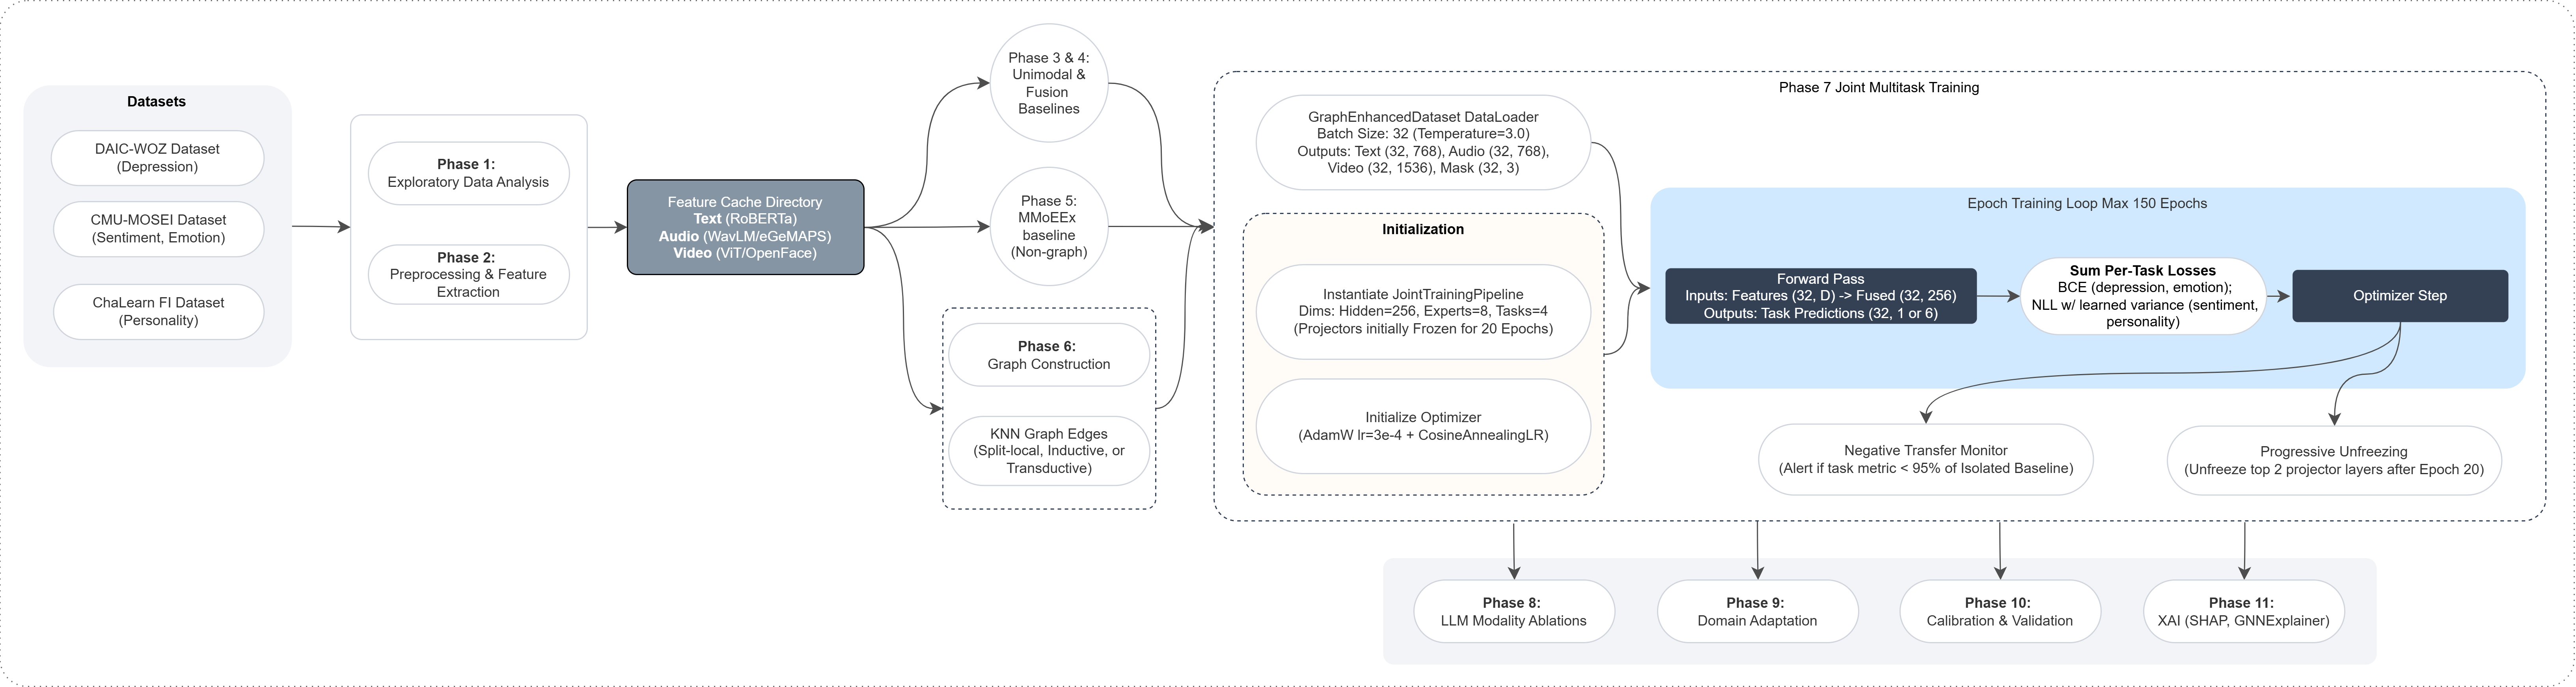
\includegraphics[width=0.85\textwidth]{figures/pipeline-flow.png}
    \caption{Implementation details of the experimental pipeline and joint multitask training. The diagram shows the progression from dataset caching through the non-graph MMoEEx baseline into the Phase 7 multitask epoch loop---including the negative-transfer monitor and progressive unfreezing mechanisms---and concluding with downstream domain adaptation, calibration, and XAI validation layers.}
    \label{fig:process_flow_main}
\end{figure*}

\section{Related Work}

\textbf{Multimodal fusion} for affective computing spans early fusion (feature concatenation), late fusion (learned per-modality gates), and low-rank or cross-attention fusion. Gated late fusion with learned modality gates \citep{hazdar2024gated} and Low-Rank Multimodal Fusion \citep{zadeh2017LMF} avoid the parameter cost of full tensor fusion. Cross-modal attention has been proposed for depression detection with a reported AUROC gain \citep{kim2024crossmodal}; we do not observe this gain under our evaluation protocol (Section~\ref{sec:results}).

\textbf{Mixture-of-experts.} The sparsely-gated MoE layer \citep{shazeer2017moe} routes inputs through a learned subset of experts. Multitask MoE (MMoE) adds task-specific gates \citep{ma2018model}, and MMoEEx adds expert exclusivity/orthogonality regularization to reduce expert collapse \citep{jacobs2024mmoe}. We build on MMoEEx and add graph-based routing.

\textbf{Graph neural networks for routing.} GraphSAGE \citep{graphsage2017inductive} learns inductive aggregator functions that generalize to unseen nodes — a requirement for clinical deployment on new participants. We use GraphSAGE (and, as an ablation, GAT \citep{gat2018attention}) as a router: aggregating features from a sample's K nearest neighbours to produce a routing vector that modulates expert weights.

\textbf{LLM-enhanced encoders.} Instruction-tuned LLMs have been applied to depression detection via text encoders \citep{zhao2025multimodalllm} and audio-language models \citep{alam2025wav2vec}. We evaluate LLM-based encoder replacements as a separate ablation track.


\textbf{Depression detection on DAIC-WOZ.} The corpus \citep{gratch2014distress} contains 189 clinical interviews with PHQ-8 labels. Reported results include Burdisso et al. GCN (F1=0.85) \citep{burdisso2024gcndp}, Zhang et al. MIL (AUROC=0.78) \citep{zhang2025mil}, Niu et al. multimodal fusion (F1=0.92) \citep{niu2021multimodal}, and Dai et al. full fusion (F1=0.96) \citep{dai2021fullfusion}. Direct comparison is limited since most prior work reports F1 while we report AUROC.

\section{Method}
\label{sec:method}

The method is intentionally conservative: we use standard multimodal encoders and MoE components so that any performance change can be attributed to graph-guided routing rather than to a novel backbone. Figure~\ref{fig:architecture} gives an overview: modality-specific encoders project to a common $d{=}256$ space; gated late fusion combines them; an MMoEEx expert bank and a KNN-graph GraphSAGE router jointly determine expert routing weights; task heads predict depression, sentiment, emotion, and personality.

\begin{figure*}[t]
    \centering
    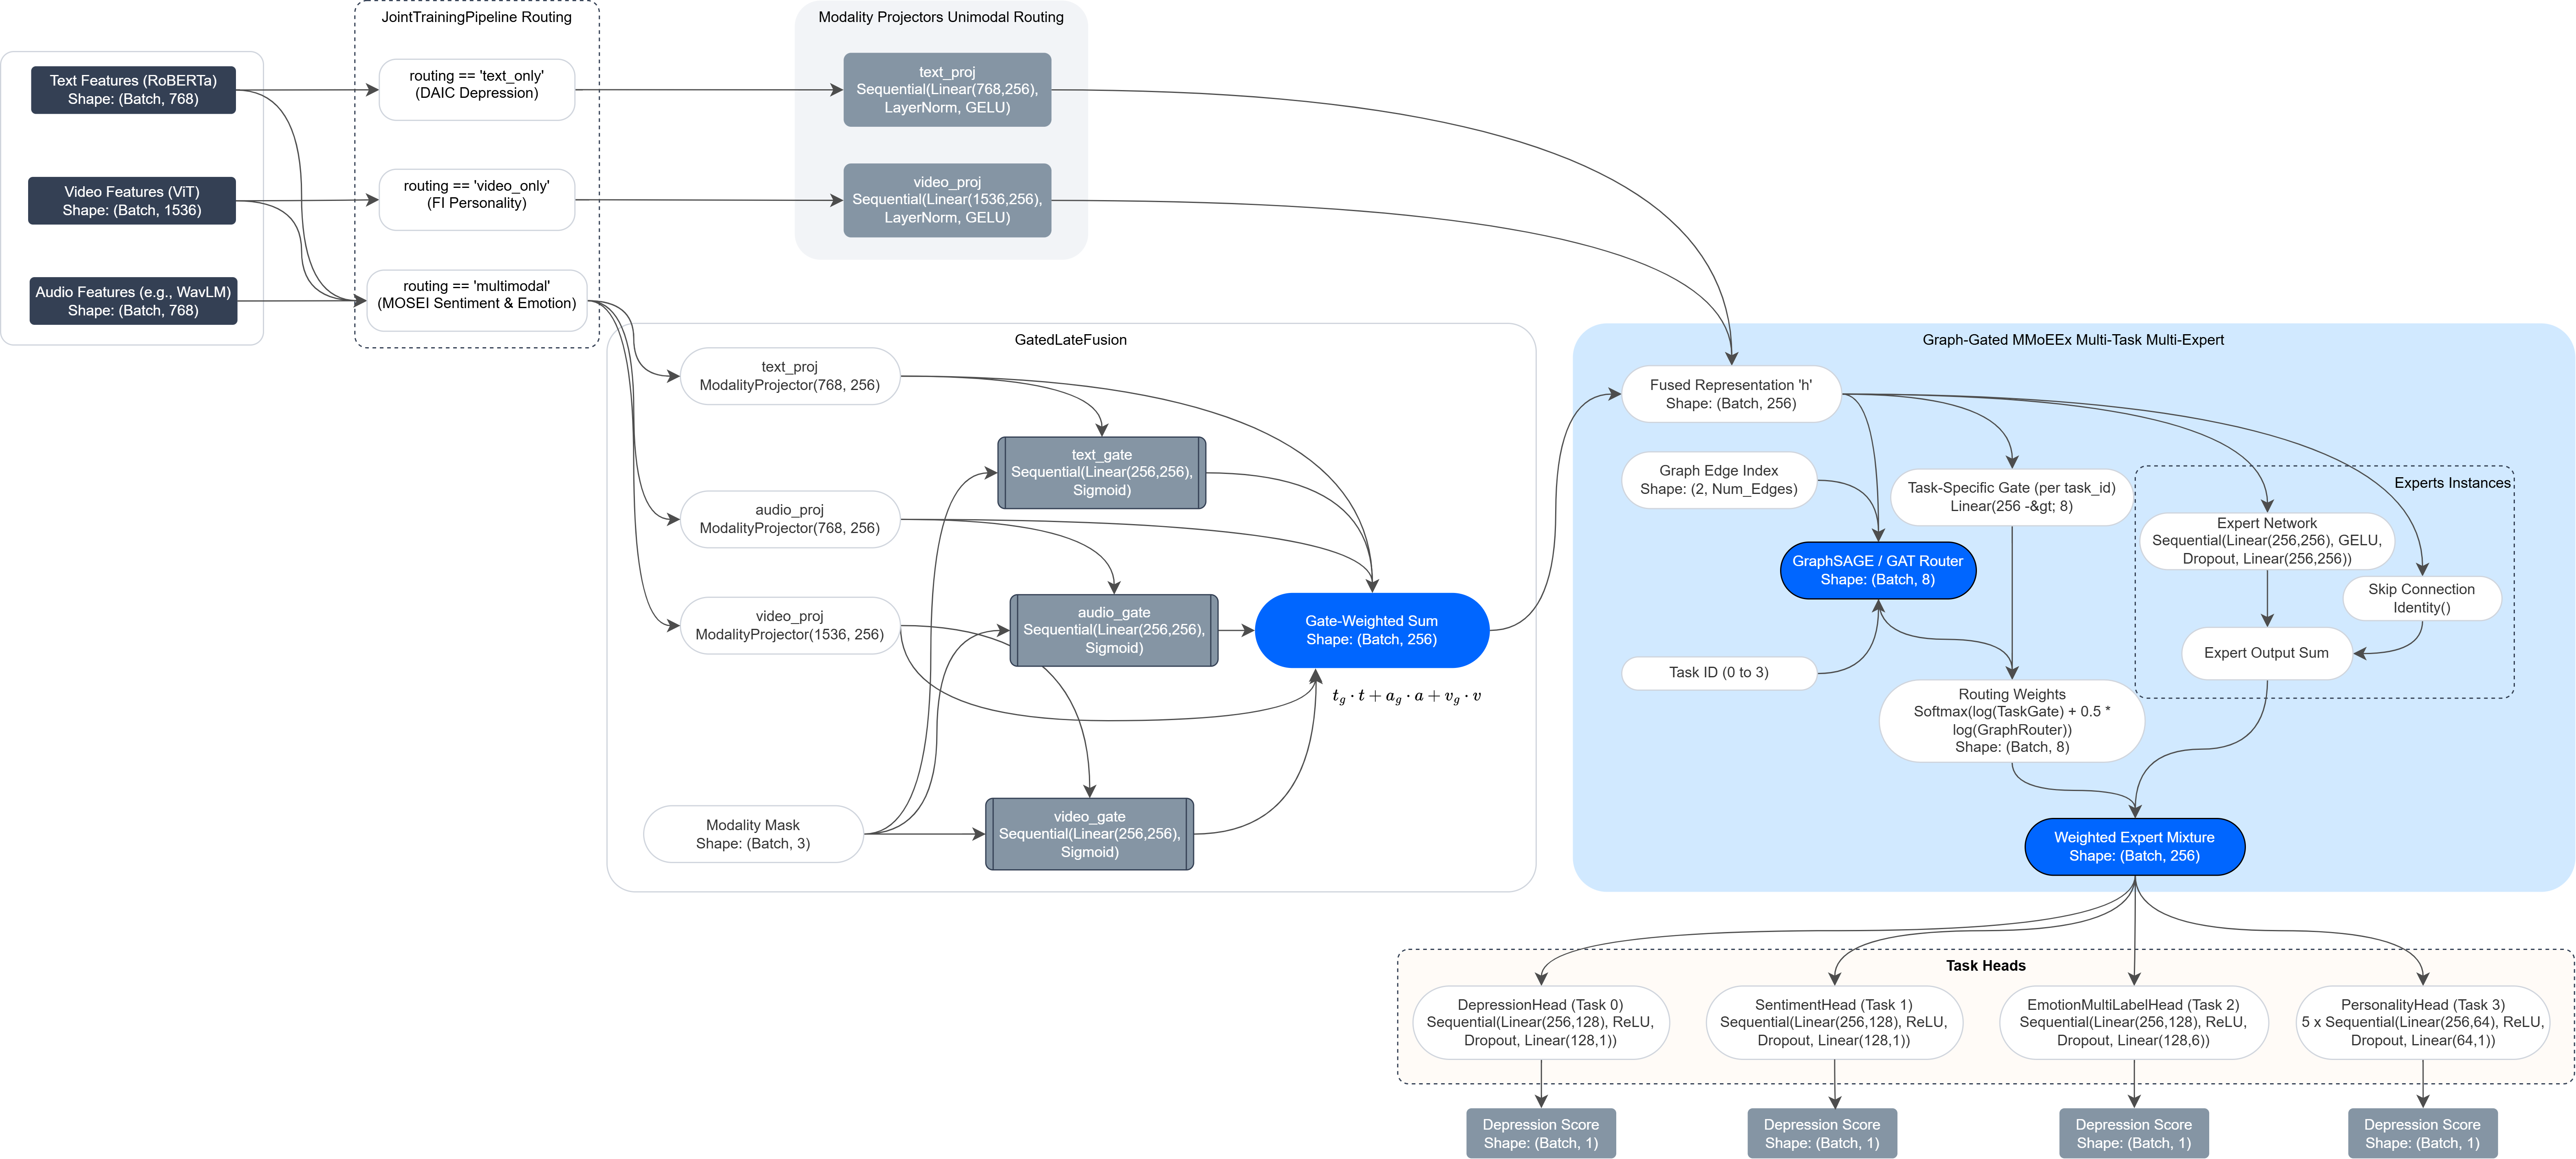
\includegraphics[width=0.85\textwidth]{figures/model_architecture.png}
    \caption{Unified multimodal graph-gated MoE architecture, including per-dataset routing, the gated fusion mechanism, the MMoEEx expert bank, and the GraphSAGE/GAT router.}
    \label{fig:architecture}
\end{figure*}

\subsection{Modality Encoders and Gated Fusion}

Text is encoded with RoBERTa-base \citep{liu2019roberta} (768-dim), audio with WavLM-large \citep{chen2022wavlm} (1536-dim; eGeMAPS \citep{eyben2016geneva} for the classical-encoder ablation), and video with ViT-B/16 \citep{dosovitskiy2020image} (1536-dim; OpenFace \citep{baltrusaitis2018openface} action units as an alternative). Each is linearly projected to $d{=}256$. Given projected embeddings $h_i^{\text{text}}, h_i^{\text{audio}}, h_i^{\text{video}}$ and a modality-availability mask $m_i$ (FI has no text; some DAIC sessions have incomplete audio), gated late fusion computes:
\begin{align*}
    \alpha_i &= \text{softmax}\big(W_\alpha[h_i^{\text{text}}; h_i^{\text{audio}}; h_i^{\text{video}}]\big), \\
    h_i^{\text{fused}} &= \sum_m \frac{\alpha_i \odot m_i}{\lVert \alpha_i \odot m_i \rVert_1 + \epsilon}[m]\, h_i^{m}.
\end{align*}

\subsection{MMoEEx Expert Bank and Graph-Guided Routing}

We instantiate $M{=}8$ expert MLPs with residual connections, hidden dimension 256 in both configurations we report. For the graph-routed configuration (our primary reported results), all 8 experts are available to every task via a full per-task softmax gate $g_t(h_i) \in \mathbb{R}^8$; we additionally report a non-graph MMoEEx baseline that hard-isolates experts per task group instead, used to quantify the value added by graph routing.

We construct an undirected KNN graph over fused embeddings using cosine similarity, with three leakage-safe construction modes: \textbf{inductive} (graph on training data only; validation/test nodes connect solely to training neighbours), \textbf{split-local} (separate graphs per split, no cross-split edges), and \textbf{transductive} (graph over all splits — ablation only, explicitly not leakage-safe). A two-layer GraphSAGE router aggregates neighbourhood features into a routing vector $r_i = \text{softmax}(W_r h_i^{(2)}) \in \mathbb{R}^8$. Task gate and graph router combine in log-space:
\[
    \tilde w_{t,i} = \text{softmax}\big(\log g_t(h_i) + \lambda \log r_i\big),
\]
with $\lambda{=}0.5$ fixed across all reported experiments (not tuned).

\subsection{Task Heads and Training Objective}

Depression (DAIC) uses a binary head with BCE loss; sentiment (MOSEI) a regression head with NLL loss; emotion (MOSEI, 6 labels) a multi-label BCE head; personality (FI, Big-Five) five regression heads with NLL loss. The multitask objective is an unweighted sum of the four task losses; the two regression losses (sentiment, personality) additionally use a homoscedastic-uncertainty NLL form \citep{kendall2017uncertainties} with a single learned $\sigma$ shared across both:
\[
    \mathcal{L} = \mathcal{L}_{\text{dep}}^{\text{BCE}} + \mathcal{L}_{\text{emo}}^{\text{BCE}} + \tfrac{1}{2\sigma^2}\big(\mathcal{L}_{\text{sent}} + \mathcal{L}_{\text{pers}}\big) + \log\sigma.
\]

\section{Experimental Setup}

\subsection{Datasets}

\textbf{DAIC-WOZ}: 189 clinical interview sessions (107 train / 35 val / 47 test), PHQ-8 binary depression label, subject-independent splits. \textbf{CMU-MOSEI} \citep{zadeh2018multimodal}: 22{,}777 utterance-level samples (16{,}265 / 1{,}869 / 4{,}643), continuous sentiment and 6-label emotion. \textbf{ChaLearn First Impressions} \citep{escalante2020chalearn}: 10{,}000 clips (6{,}000 / 2{,}000 / 2{,}000), Big-Five apparent-personality regression; personality is a distinct construct from clinical depression and serves as auxiliary supervision only.

\subsection{Training Details}

AdamW ($\text{lr}{=}3\times10^{-4}$), cosine annealing, early stopping (patience 20 epochs, max 150). Batch size 32. Temperature-balanced sampling ($T{=}3.0$) prevents MOSEI (120$\times$ larger than DAIC) from dominating joint training. Projectors are frozen for the first 20 epochs, then the top 2 layers are unfrozen.

\subsection{Evaluation}

DAIC: AUROC (primary) and F1. MOSEI sentiment: CCC (primary). MOSEI emotion: macro-AUROC over 6 emotions. FI: mean CCC over five traits. All results report 95\% BCa bootstrap confidence intervals; AUROC comparisons use the DeLong test; CCC/F1 comparisons use paired permutation tests; effect sizes are Cohen's $d$.

\section{Results}
\label{sec:results}

\begin{table}[t]
    \centering
    \caption{Graph routing vs.\ non-graph MMoEEx baseline, real labels and evaluation throughout. Best per-column among graph variants in \textbf{bold}; baseline row is the reference, not part of the ablation.}
    \label{tab:graph_ablation}
    \small
    \begin{tabular}{lccc}
        \toprule
        Variant                 & DAIC AUROC     & MOSEI CCC      & FI CCC                \\
        \midrule
        \emph{Non-graph MMoEEx} & \emph{0.493}   & \emph{0.493}   & \emph{\textbf{0.578}} \\
        \midrule
        V0 (inductive-k10)      & 0.515          & \textbf{0.517} & 0.542                 \\
        V1 (split-local-k10)    & \textbf{0.551} & 0.514          & 0.542                 \\
        V2 (transductive-k10)   & 0.507          & 0.515          & 0.553                 \\
        V3 (inductive-k15)      & 0.525          & 0.510          & 0.544                 \\
        V4 (split-local-k15)    & 0.540          & 0.511          & 0.540                 \\
        \bottomrule
    \end{tabular}
\end{table}

\begin{figure}[t]
    \centering
    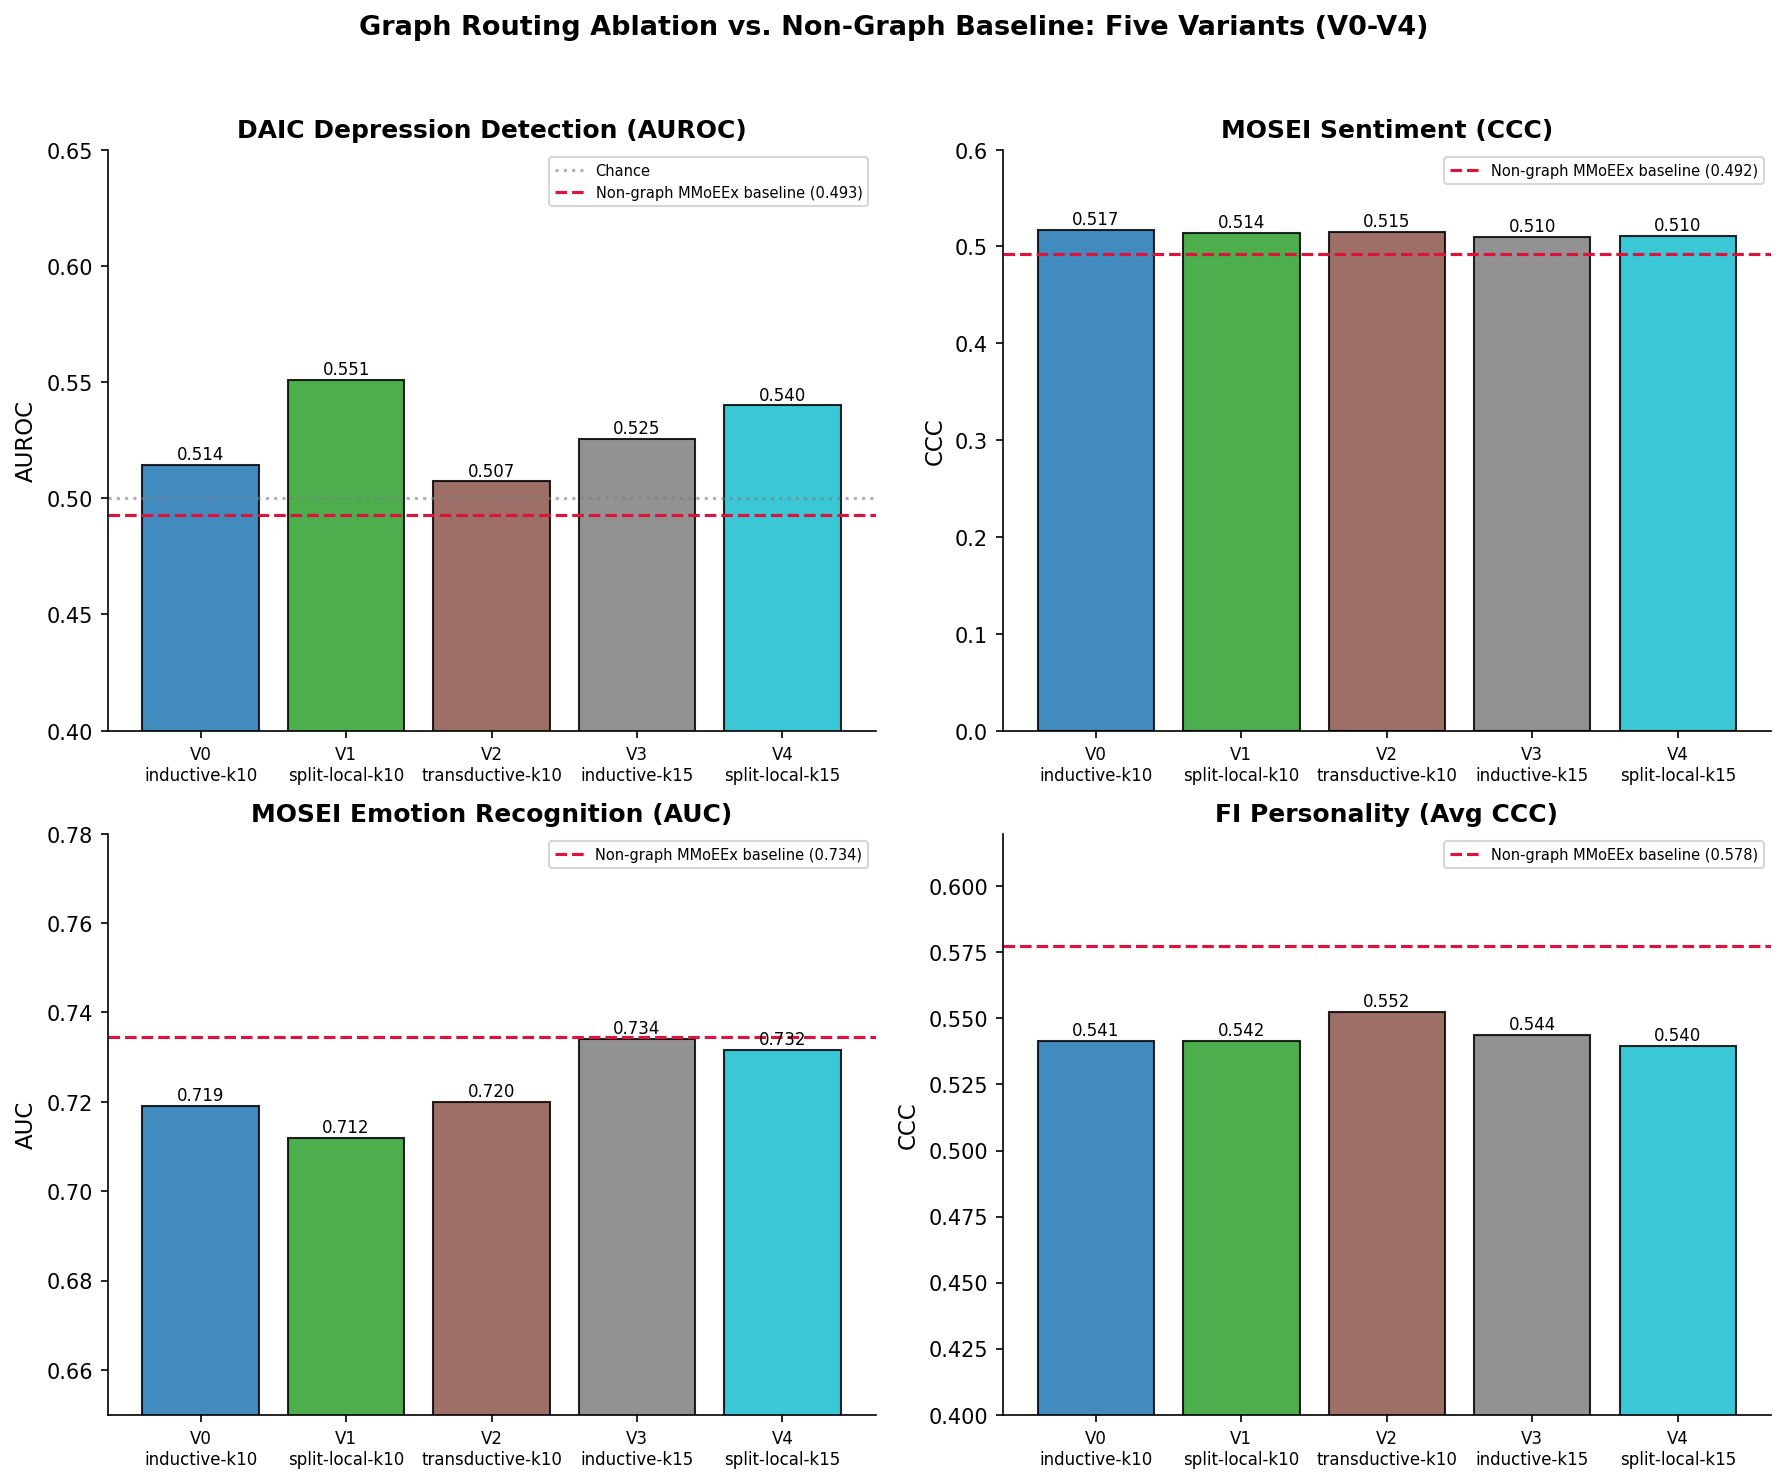
\includegraphics[width=\columnwidth]{figures/graph_ablation.png}
    \caption{Graph routing vs.\ non-graph baseline (red dashed line). Small, inconsistent edge on DAIC/MOSEI; consistently below baseline on FI.}
    \label{fig:graph_ablation_main}
\end{figure}

Every graph-routed variant is within bootstrap-CI-width of the non-graph baseline on DAIC and MOSEI, and every variant underperforms the baseline on FI personality. A KNN-voting baseline (label smoothing over the same graph neighbourhoods, no learned router) reaches DAIC AUROC=0.630 — higher than every learned graph-routed variant. A homophily diagnostic (same-dataset edge label agreement/correlation vs.\ random pairing, Table~\ref{tab:homophily}) explains this differently per task: DAIC's routing graph carries no signal beyond chance, while MOSEI and FI both carry real signal the router fails to exploit.

\begin{table}[t]
    \centering
    \caption{Real graph neighbours vs.\ random pairing (val split, averaged over 4 leakage-safe variants).}
    \label{tab:homophily}
    \small
    \begin{tabular}{lcc}
        \toprule
        Task                   & Real graph & Random baseline \\
        \midrule
        DAIC (label agreement) & 0.568      & 0.555           \\
        MOSEI (correlation)    & 0.249      & $-$0.006        \\
        FI (correlation)       & 0.279      & $-$0.002        \\
        \bottomrule
    \end{tabular}
\end{table}

\begin{figure}[t]
    \centering
    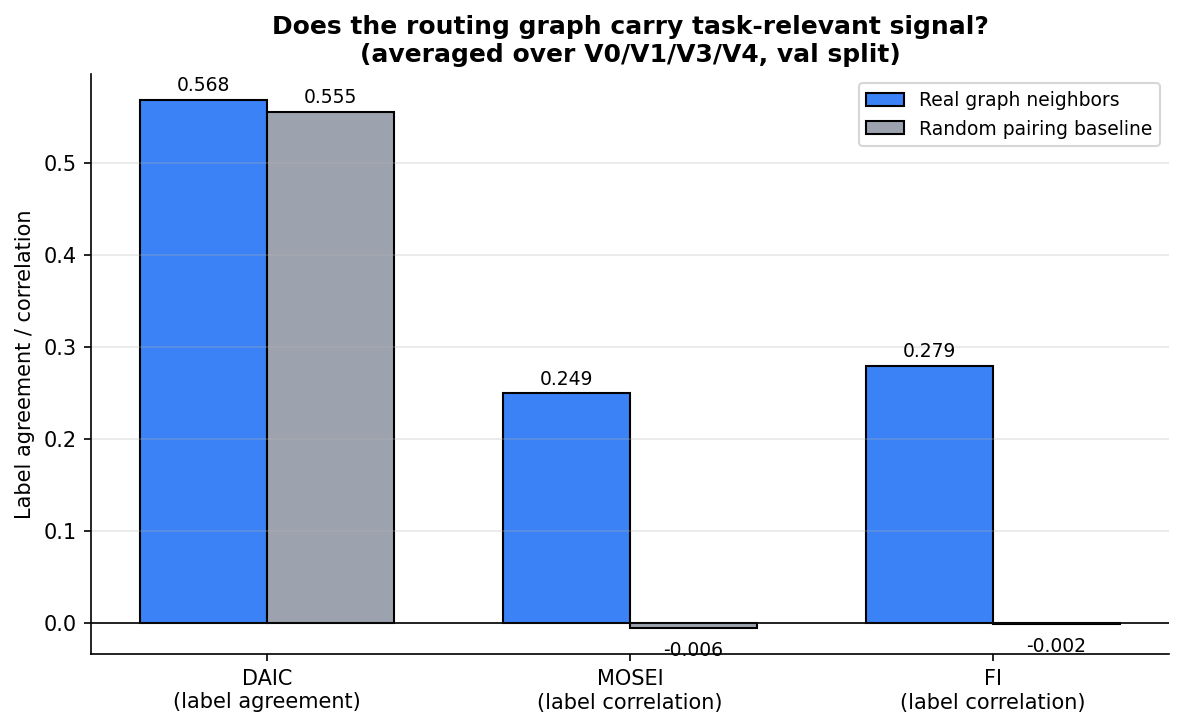
\includegraphics[width=\columnwidth]{figures/09_graph_homophily_diagnostic.png}
    \caption{Real graph neighbours vs.\ random pairing, averaged over V0/V1/V3/V4. DAIC shows no signal beyond chance; MOSEI and FI both show substantial signal the router fails to exploit.}
    \label{fig:homophily}
\end{figure}

Two targeted fixes did not recover a benefit: a $K\in\{5,10,15,20\}$ sweep shows no monotonic trend (Appendix, supplementary material), and a learned per-task routing weight (replacing the fixed $\lambda{=}0.5$) moved in the direction the diagnostic predicts (down for FI/MOSEI-emotion, up for MOSEI-sentiment) but only slightly ($\pm0.07$), with DAIC AUROC improving to 0.544 and FI CCC unchanged at 0.541.

On fusion, cross-attention underperforms gated fusion on all three datasets and does not reproduce a previously reported +0.041 AUROC gain \cite{kim2024crossmodal}, likely due to overparameterization (65K--2.8M params vs.\ 57K--827K for gated) relative to DAIC's 107 training sessions.

\subsection{LLM-Enhanced Encoders (L0--L5)}
\label{sec:llm_ablation}

We replace classical encoders with LLM-based encoders at each modality: \textbf{L0} classical baseline (RoBERTa+WavLM+OpenFace); \textbf{L1} Mistral-7B-Instruct-v0.3 frozen text encoder; \textbf{L2} L1 with a LoRA ($r{=}16$, $\alpha{=}32$) trainable adapter; \textbf{L3} L1 + CLAP audio encoder; \textbf{L4} L1 + LLaVA-1.5-7B video encoder; \textbf{L5} the full LLM stack (text+audio+video replaced).

\begin{table}[t]
    \centering
    \caption{Best LLM-ablation level per headline metric vs.\ classical (L0) baseline. Every level improves over L0 on every metric; shown is each metric's best level.}
    \label{tab:llm_ablation}
    \small
    \begin{tabular}{lccc}
        \toprule
        Metric                & Best level & Value  & $\Delta$ vs.\ L0 \\
        \midrule
        DAIC AUROC             & L3 (Mistral+CLAP) & 0.7210 & $+$0.174 \\
        MOSEI emotion AUROC    & L1 (Mistral text) & 0.7702 & $+$0.147 \\
        MOSEI sentiment CCC    & L5 (full stack)   & 0.6284 & $+$0.089 \\
        FI personality CCC     & L2 (Mistral+LoRA) & 0.5732 & $+$0.115 \\
        \bottomrule
    \end{tabular}
\end{table}

\begin{figure}[t]
    \centering
    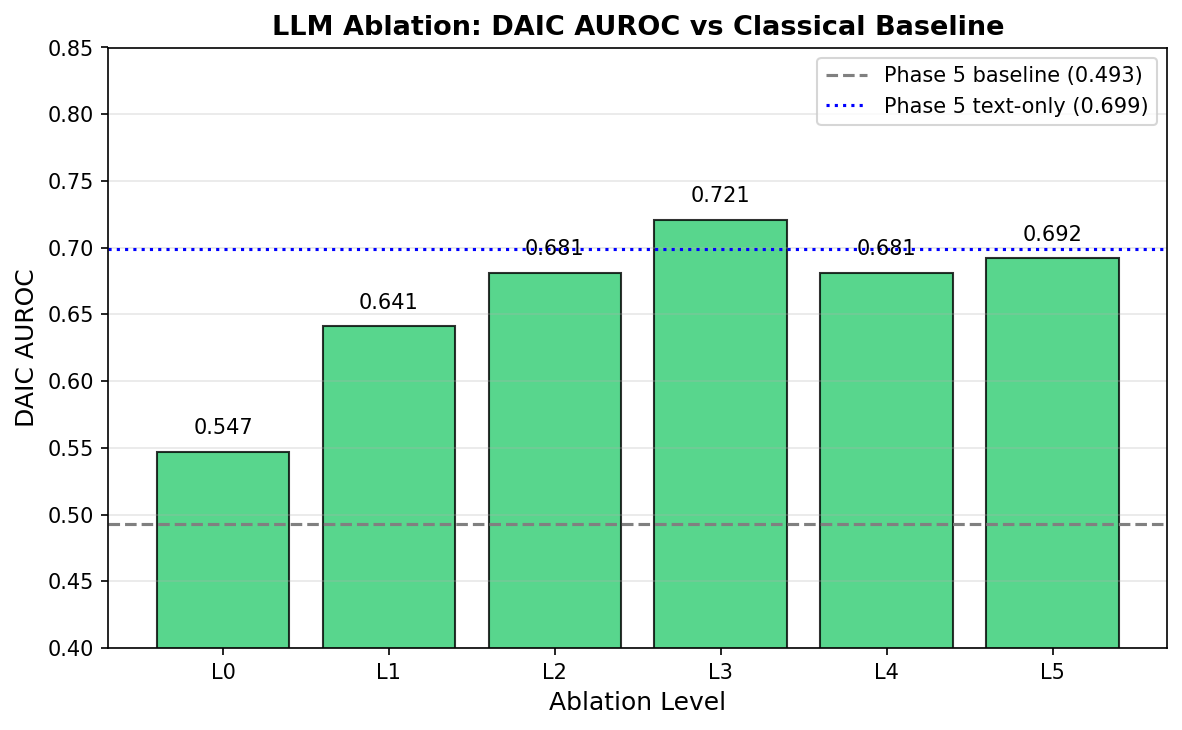
\includegraphics[width=\columnwidth]{figures/llm_delta_bar.png}
    \caption{LLM modality ablation: DAIC AUROC per level (L0--L5) against the classical (L0) and Phase-5 text-only baselines. L3 (Mistral+CLAP) gives the largest gain.}
    \label{fig:llm_ablation_delta}
\end{figure}

Every LLM level improves over the classical baseline on all three headline metrics, and every LLM level substantially outperforms every graph-routed variant on every metric (e.g.\ L3 DAIC AUROC 0.7210 vs.\ the best graph variant's 0.5507) — across our experiments, encoder quality produced larger gains than routing changes. L4 (Mistral+LLaVA) shows a validation/test gap traced to an audio feature-dimension mismatch between its training checkpoint and the inference dataset; we report this as a known limitation rather than a representative L4 result (supplementary material).

\subsection{Domain Adaptation}
\label{sec:domain_adaptation}

We tested unsupervised domain adaptation (CORAL, MMD, DANN, and a combined CORAL+MMD loss) for transferring FI and MOSEI representations to DAIC depression detection, against a no-adaptation baseline, across three transfer scenarios (FI$\to$DAIC, MOSEI$\to$DAIC, multisource). All four methods underperform the no-adaptation baseline in 10 of 12 evaluated conditions: the no-adaptation baseline's best result (MOSEI$\to$DAIC, AUROC=0.6942) beats the best DA result anywhere (combined CORAL+MMD, FI$\to$DAIC, AUROC=0.6901); CORAL is the most consistently harmful ($-$0.0744 vs.\ baseline at worst), and only MMD marginally improves its own no-adaptation baseline (+0.0041, within bootstrap CI). We attribute this to DAIC's training set ($n{=}107$) being too small to train a stable domain discriminator, and to shared multitask heads already providing implicit alignment; we do not merge domain adaptation into the main model.

\subsection{Generalization: Cross-Dataset Transfer (MPDD)}
\label{sec:mpdd}

To probe whether our findings generalize beyond DAIC/MOSEI/FI, we ran a supplementary benchmark on MPDD (Multimodal Depression Detector: Wav2Vec2 + OpenFace features, two age tracks). On MPDD-Young, a strongly-regularized logistic regression (AUROC=0.674) outperforms both GGMoE with and without graph routing (0.545/0.559) — the small sample size favors a linear model over any neural architecture we tested, including the graph router.

\begin{figure}[t]
    \centering
    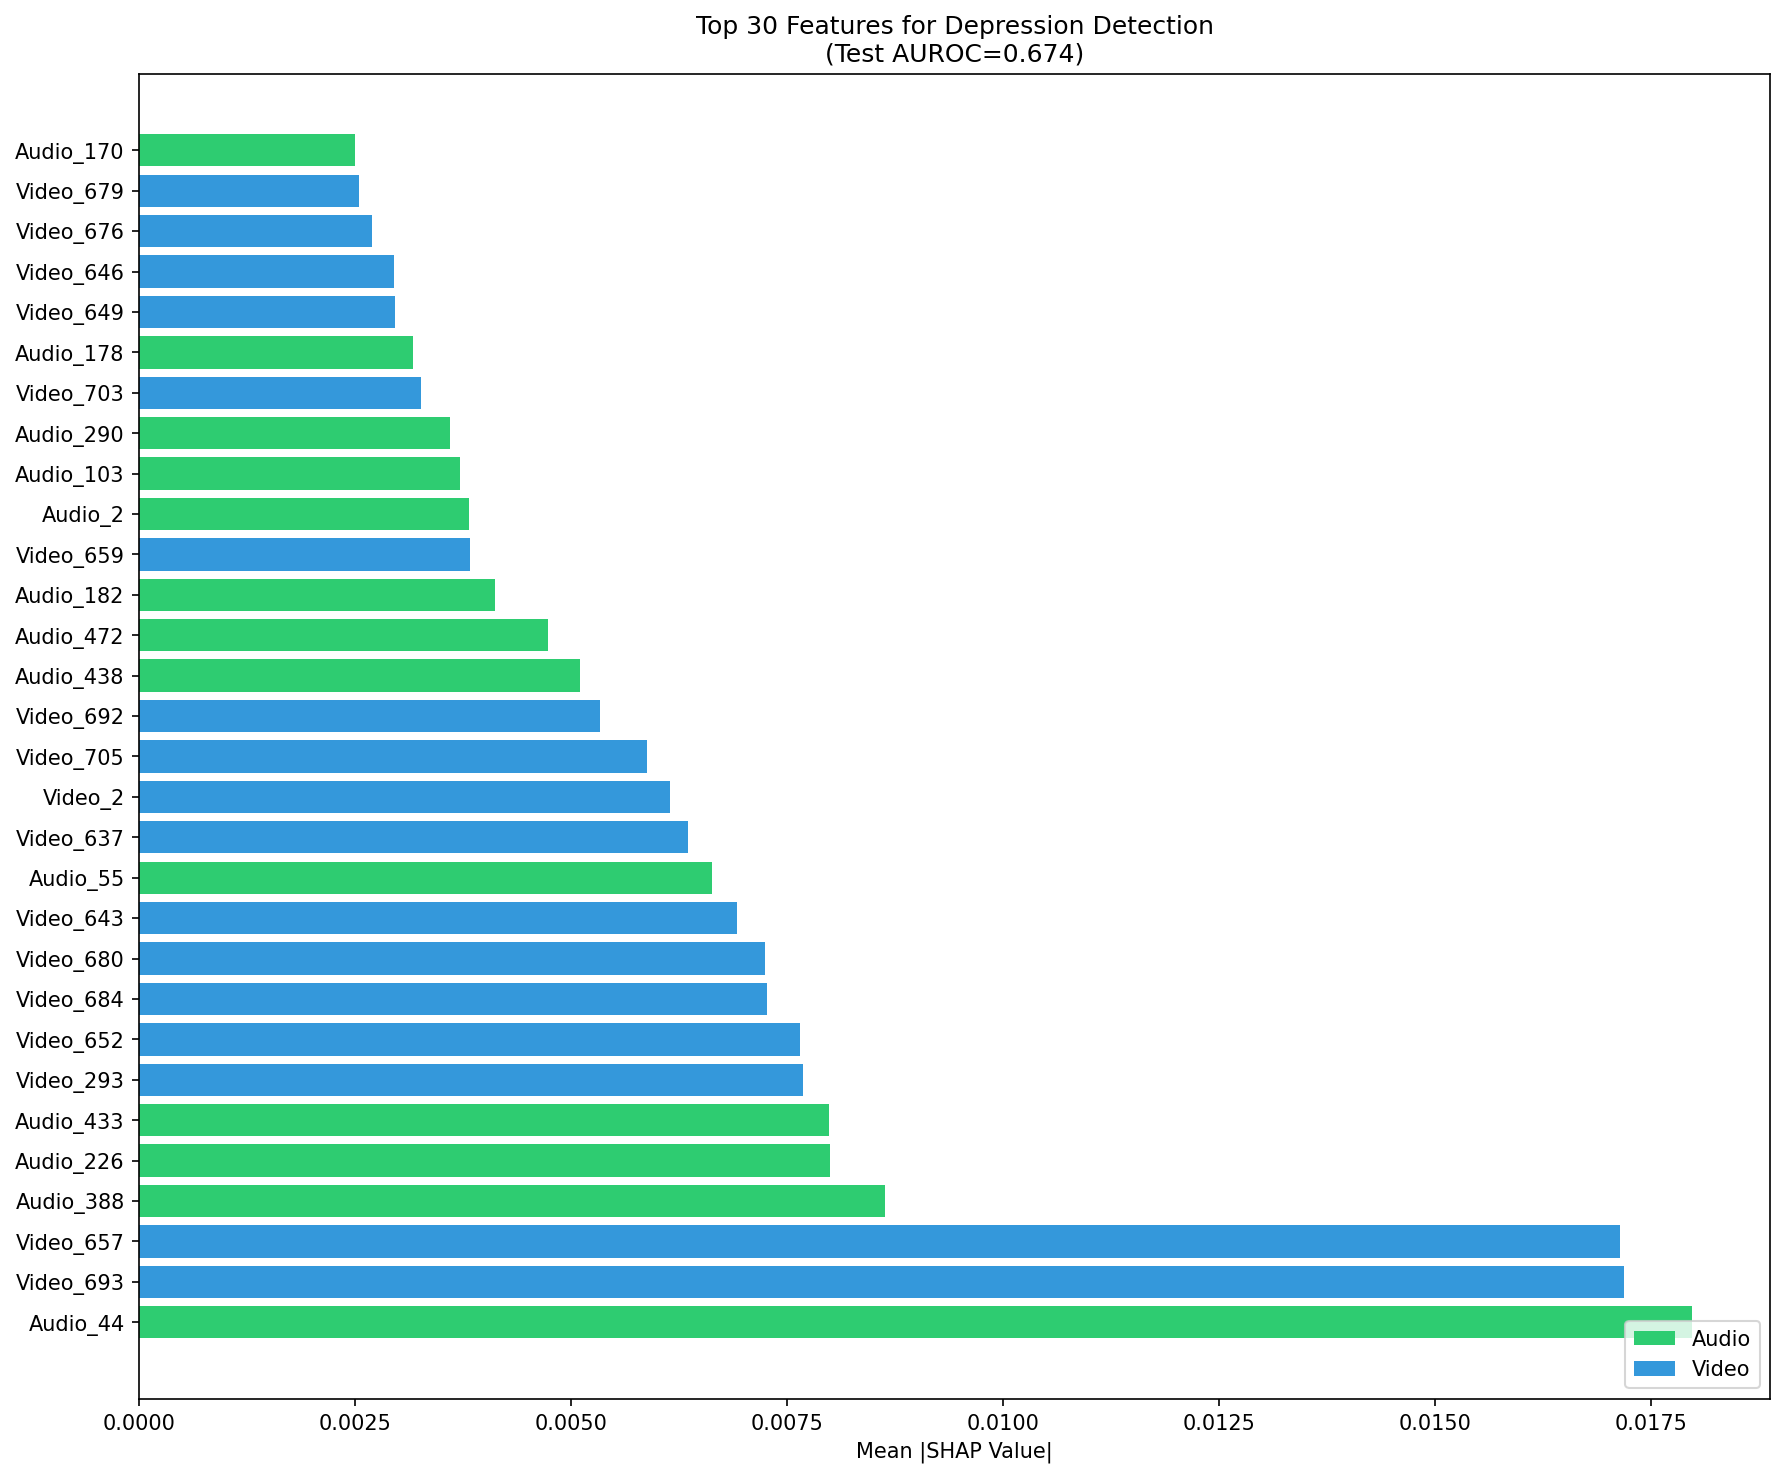
\includegraphics[width=\columnwidth]{figures/feature_importance.png}
    \caption{Top-30 SHAP feature importances for MPDD-Young depression detection. \texttt{audio\_44} is the single most important feature, though the top-30 set is video-dominated (17 of 30).}
    \label{fig:mpdd_shap_main}
\end{figure}

Zero-shot transfer from Young to Elderly collapses to near-constant predictions (cross-track AUROC=0.395, below chance), while cross-\emph{dataset} transfer sharing a Wav2Vec2-family audio encoder (MPDD$\to$DAIC) transfers positively (AUROC=0.551, above the within-DAIC baseline of 0.344) — encoder-family match appears to matter more than domain similarity for transfer, and age-group-specific rather than universal biomarkers likely explain the cross-track failure.

\section{Calibration and Statistical Validation}
\label{sec:calibration}

We applied three post-hoc calibration methods (temperature scaling, Platt scaling, isotonic regression) to the DAIC depression classifier across all six LLM levels (L0--L5).

\begin{figure}[t]
    \centering
    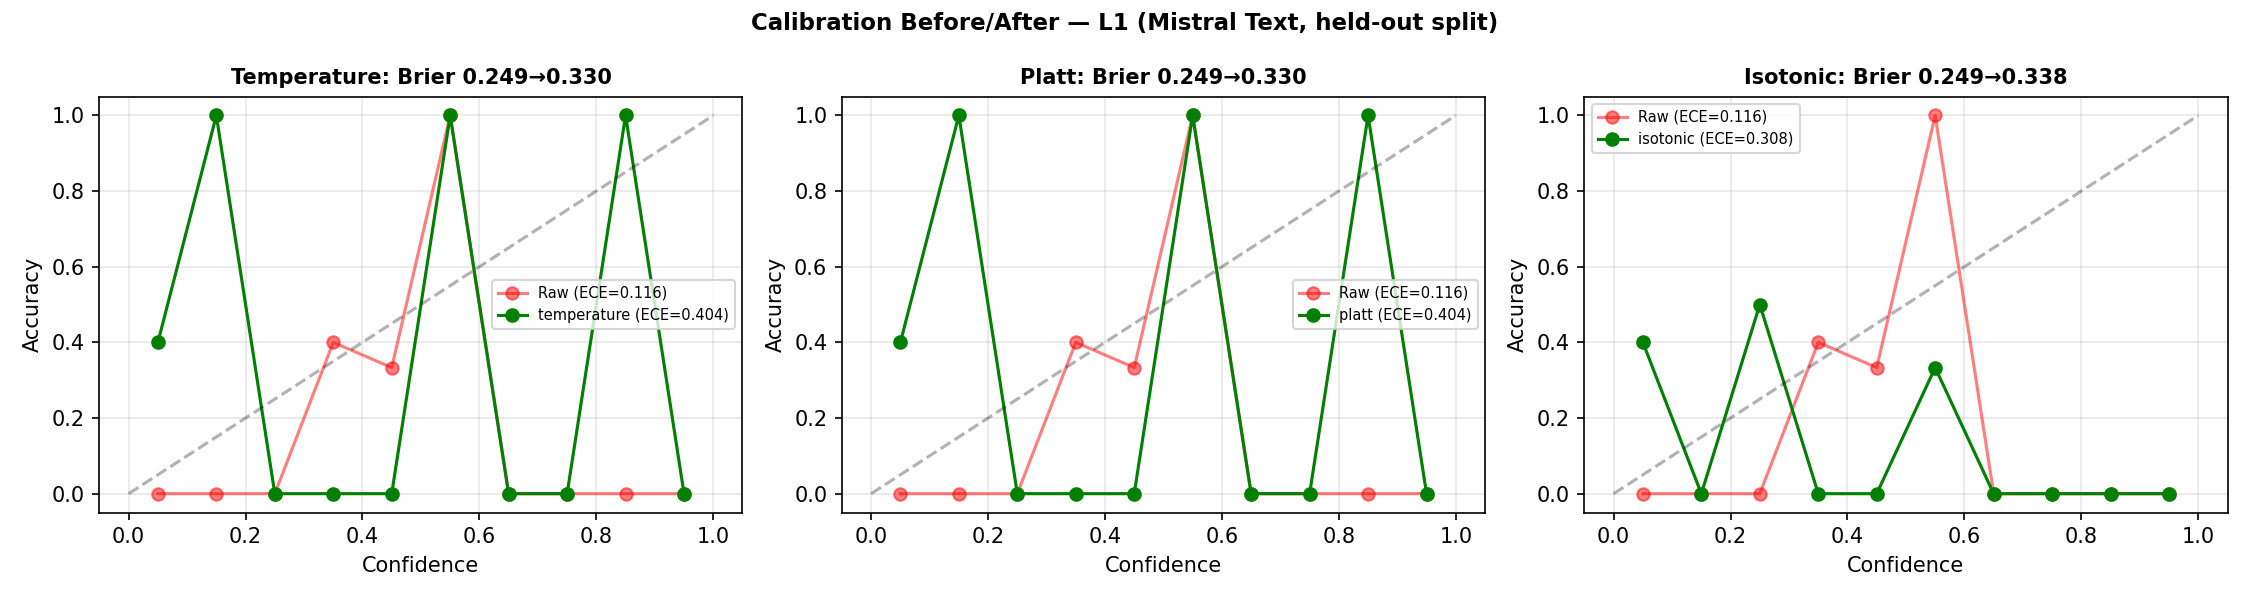
\includegraphics[width=\columnwidth]{figures/calibration.png}
    \caption{Calibration reliability diagrams (temperature/Platt/isotonic scaling vs.\ raw) for the L1 (Mistral text) DAIC classifier, held-out split. Monotonic recalibration changes reliability but not ranking-based discrimination.}
    \label{fig:calibration_main}
\end{figure}

Uncalibrated logits show moderate calibration error (ECE=0.26--0.35). Isotonic regression reduces ECE the most on held-out validation data, followed by Platt and temperature scaling; Brier score improves from 0.21--0.24 (uncalibrated) to 0.05--0.16 (calibrated). All three methods are monotonic transforms of the score, so AUROC is unchanged by temperature/Platt scaling and only marginally affected by isotonic regression's tie-breaking — calibration improves probabilistic reliability without altering discrimination, which matters if predicted probabilities (not just rankings) inform a clinical threshold.

We report every headline metric with BCa bootstrap confidence intervals (2,000 resamples), the DeLong test for AUROC comparisons, paired permutation tests (10,000 sign-flips) for F1/CCC/MAE comparisons, and Cohen's $d$ effect sizes. Across all LLM ablation pairs (L1--L5 vs.\ L0), no comparison reaches significance at $\alpha=0.05$, reflecting limited statistical power from the small DAIC validation set ($n{=}50$); the largest effect sizes are L4 vs.\ L0 ($d=0.170$) and L1 vs.\ L0 ($d=0.152$). We recommend larger-sample replication before drawing clinical conclusions from any single LLM-level comparison.

\section{Explainability}
\label{sec:xai}

Section~\ref{sec:method} motivated two transparency mechanisms alongside the routing-performance question above: characterizing depression jointly with sentiment, emotion, and personality rather than as an isolated score, and using the routing graph as a source of visual and machine-readable explanation. We evaluate both directly on real validation instances rather than only asserting they are implemented.

\begin{figure}[t]
    \centering
    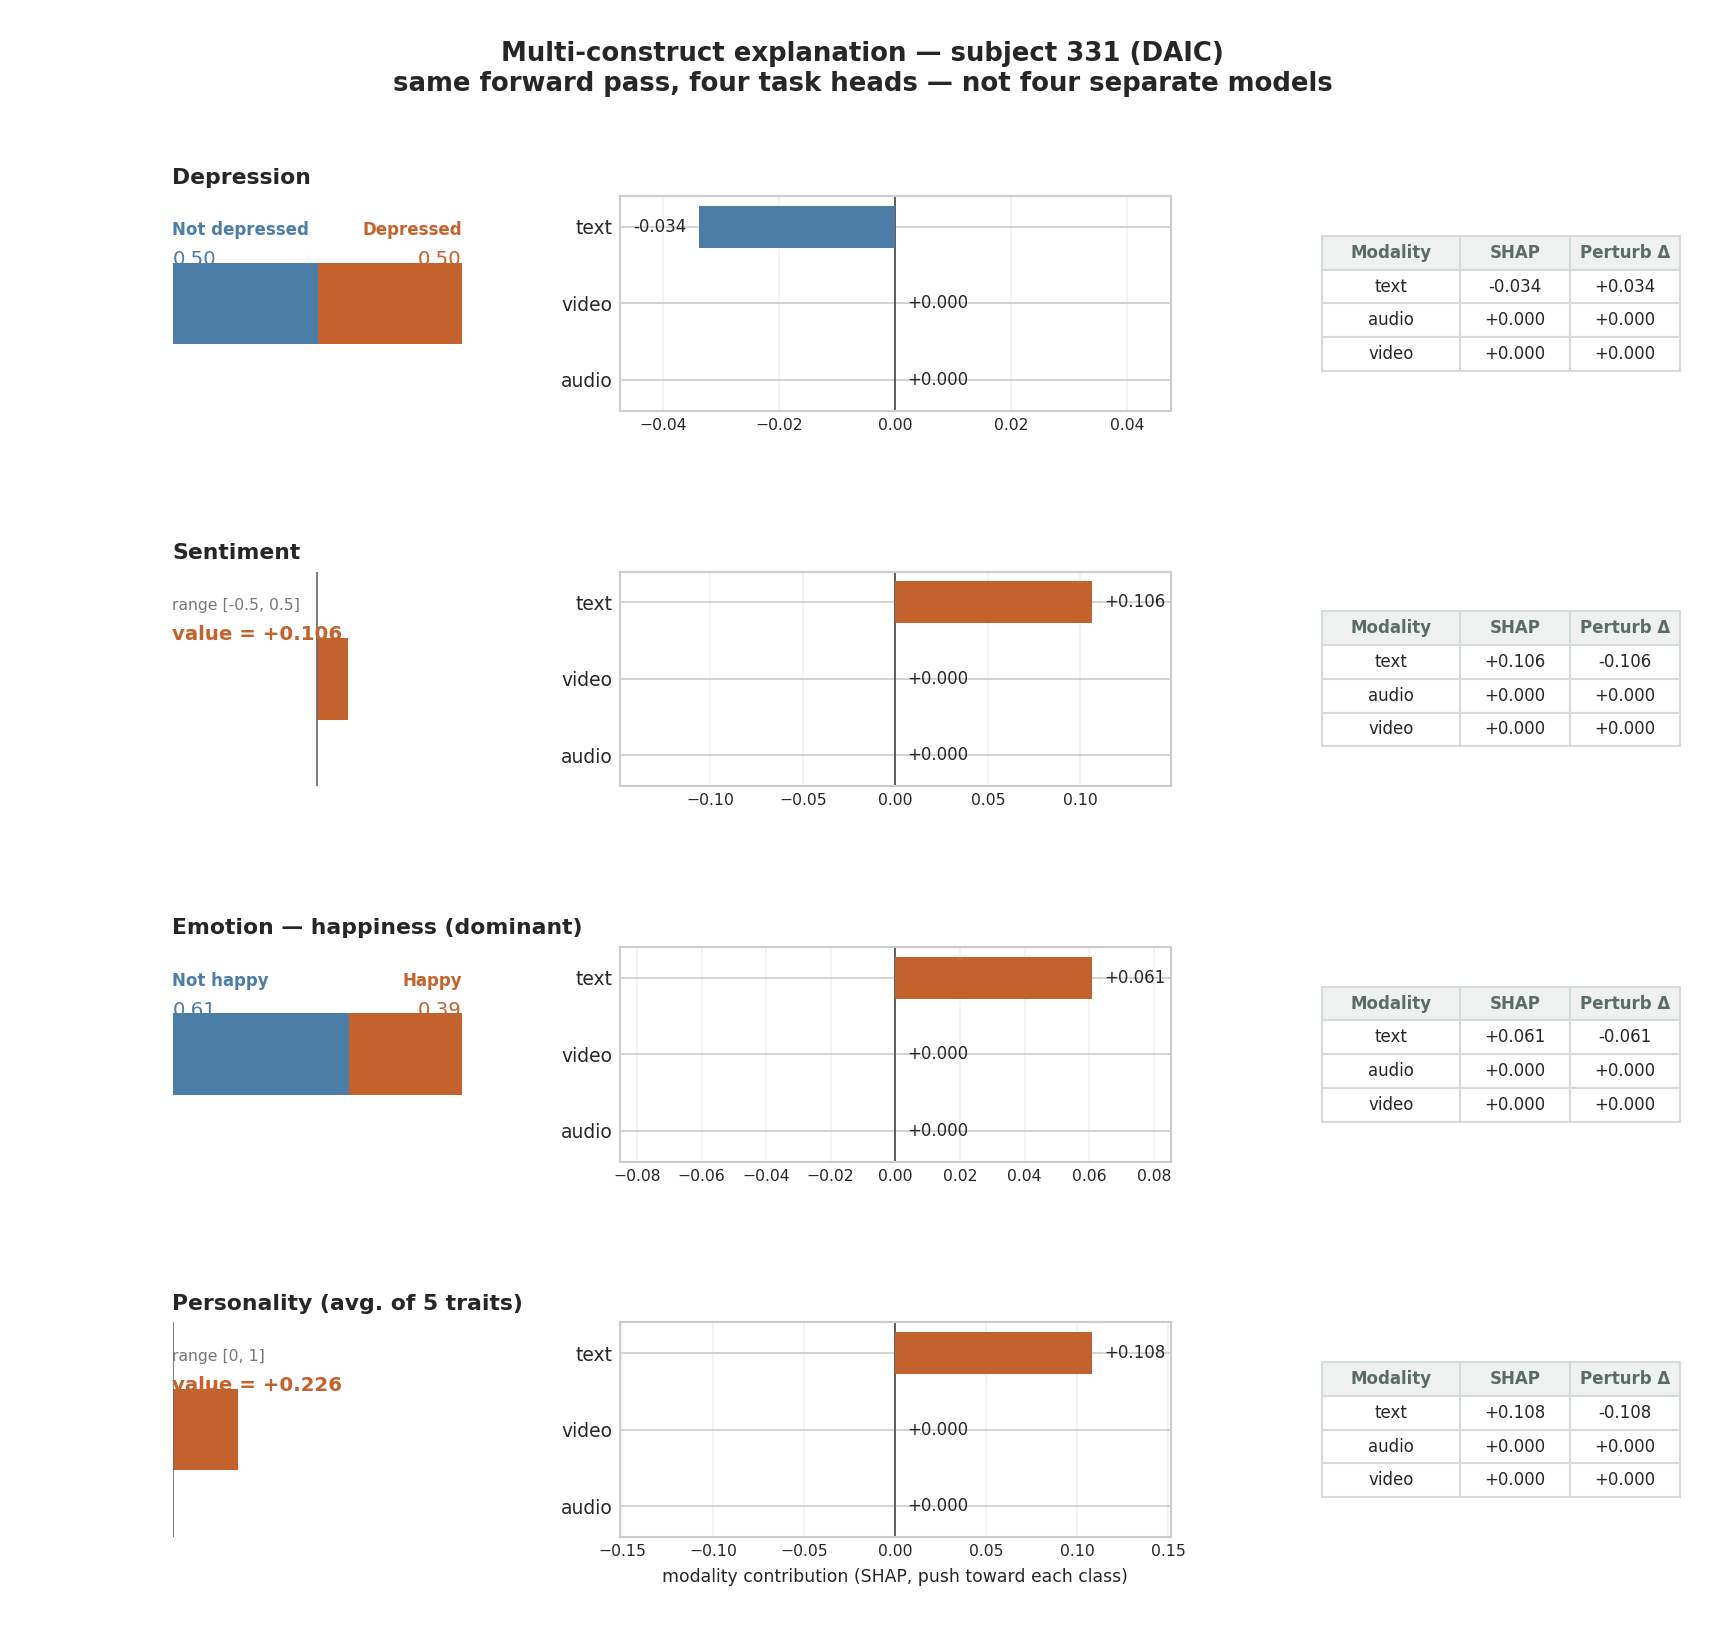
\includegraphics[width=\columnwidth]{figures/daic_multi_construct_force.png}
    \caption{Multi-construct explanation for one DAIC subject: the same forward pass, explained through all four task heads. Audio and video read exactly zero on every row, directly visualizing DAIC's text-only routing (Section~\ref{sec:method}) rather than leaving it implicit.}
    \label{fig:multi_construct_main}
\end{figure}

For the first mechanism, we pass each sample's shared representation through all four task heads in one forward pass, not only the head matching its own source dataset. On a representative MOSEI case this profile is sharply coherent (happiness probability 0.89, sentiment $+0.62$, sadness/anger/fear all below 0.09); on DAIC, Figure~\ref{fig:multi_construct_main} shows every head's SHAP attribution is exactly zero for audio and video and driven entirely by text, which is the correct, faithful behaviour given DAIC's text-only routing rather than an artefact — a modality outside a dataset's native routing contributes nothing to any task head evaluated on it, and the profile should be read accordingly.

For the second mechanism, each case study pairs a visual record (SHAP attribution, GNNExplainer subgraph, GraphXAIN natural-language narrative) with a machine-readable one (structured SHAP values, neighbour identities and distances, routing weights). This is faithful to what the model computes but not unconditionally informative: rebuilding the explanation graph from the model's own trained representation does not improve DAIC label homophily (0.463 trained vs.\ 0.537 random vs.\ 0.577 raw features, on the 35 DAIC validation samples), so DAIC subgraph explanations should be read as showing which samples the model geometrically treats as similar, without a validated claim that those neighbours are similar in a depression-relevant sense. MOSEI and FI do not share this limitation (Table~\ref{tab:homophily}). We also find that LLM-generated narratives invent specific clinical detail (e.g.\ a quoted patient response) not present anywhere in their prompt, which contains only SHAP scalars, neighbour indices, and a dataset label — a concrete, reproducible instance of the risk that post-hoc clinical narratives can be fluent without being grounded \cite{wu2025cotfails}, reported here as an honest limitation of the explanation pipeline rather than a resolved property of it (supplementary material).

\section{Discussion}

The leakage-safe graph protocol is essential regardless of whether graph routing helps: transductive (non-leakage-safe) construction is retained only as an ablation, with each edge's split membership determined by direct lookup of the destination node's split label rather than an assumption about how samples are ordered in memory.

Limitations include DAIC's small training set ($n{=}107$), which limits statistical power for all pairwise comparisons; reliance on frozen pretrained encoders; sensitivity to graph quality when modalities are missing; and that our two fix attempts do not exhaust the candidate remedies the homophily diagnostic suggests (a jointly-trained or contrastively-pretrained embedding space for graph construction, graph rewiring/structure learning, and task-affinity-aware expert grouping remain untried; supplementary material).

\section{Conclusion}

For small-sample multimodal mental-health datasets with leakage-safe graphs, graph-guided routing was not beneficial in our experiments; future gains may require jointly learned graph structure, better embeddings for neighbor construction, or task-aware expert grouping. A homophily diagnostic localizes why, giving future work on graph-based routing in low-resource clinical settings a concrete starting point rather than an unexplained null result. We observe in these experiments that the most consistent gains came from encoder changes rather than routing architecture.

\bibliography{references/references}
\end{document}
